\chapter{State of the art} 

\section{Requirements}
One can notice that elements that yields a solution for a problem stated in the first chapter, which is ensuring that users' application provide appropriate Quality-of-Service for its customers in a most-cost effective manner, were gradually introduced in previous chapters:

\begin{itemize}
	\item \emph{scalability} - ability to improve application performance by enriching resources
	\item \emph{adaptivity} - ability to adapt (i.e. scale) appropriately to a current usage pattern
	\item \emph{inter-cloud awareness} - ability to compose an application deployment using different cloud providers; cooperation with different cloud provider to supply application with extra resources while performing application scaling
\end{itemize}

Next section states the general overview of the proposed solution, while the consecutive sections details its elements and finally the last section summarises the design choices in a context of system requirements.
	
% radek
\section{Carina}

\subsubsection{Overview}
Carina is an open source project, released under Apache License 2.0, built on top of OpenNebula, which aims to ``(\ldots) standardize the process for automating multi-VM deployments and setting auto-scaling and availability management policies in the cloud.'' \cite{CarinaBlog}.
As it is stated in the requirements of the solution, \emph{Carina} should support variety of features which can be considered worth scrutinizing carefully as they are closely related to notions of adaptivity and scalability. To name the most relevant: \cite{CarinaBlog}
\begin{itemize}
  \item Collect and aggregate OS or app-specific metrics across a cluster
  \item Drive elastic scaling of clusters based on workload or events
  \item Support deployment and handling of failover of services across multiple datacenters
\end{itemize}

Before delving into a more detailed discussion of these features, it is essential to introduce some Carina-specific concepts and look at the product's design and its components.

\subsection{Design}
Here are some terms used by \emph{Carina}:
\begin{itemize}
  \item Environment -- a collection of VMs in a master-slave configuration,
  \item Service -- a consumer of cloud resources. Each service can have its own environment configurations and create environments and control them independently of other services,
  \item Pools -- various clusters or virtual data centers in OpenNebula that can be targets for creating an environment
\end{itemize}

\begin{figure}[!ht]
  \begin{center}
    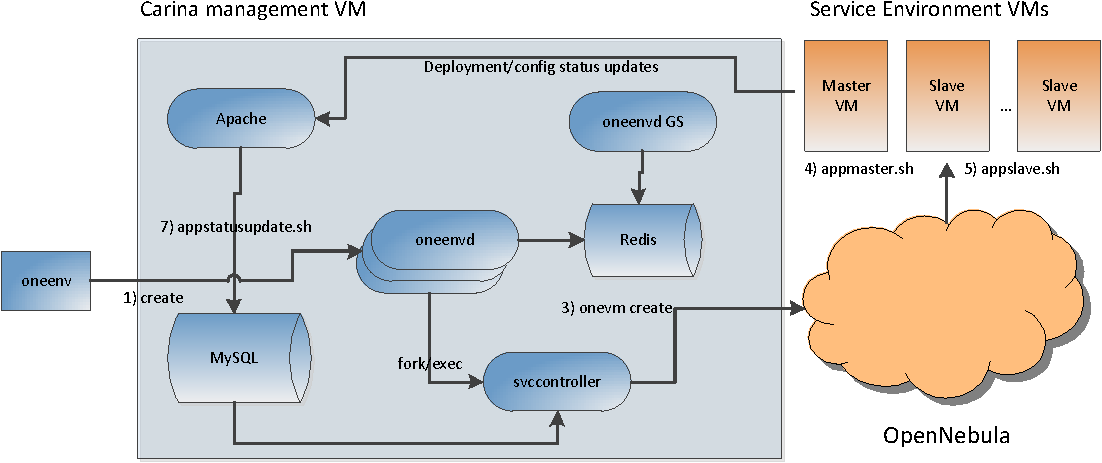
\includegraphics[width=0.9\textwidth]{state-of-the-art/carina-design}
  \end{center}
  \caption{Carina -- components interaction}
  \label{sota:carina-design}
\end{figure}

Adaptivity

Scaling
- vertical
- horizontal

Limitations

\section{OneFlow}

\section{OpenShift}

% radek
\section{CloudFoundry}



% radek
\section{Providers comparison}
	
